\documentclass[11pt,a4paper]{article}

% ---------- Codificación y fuentes ----------
\usepackage[utf8]{inputenc}
\usepackage[T1]{fontenc}
\usepackage{lmodern}
\usepackage[spanish,es-nodecimaldot]{babel}
\usepackage{microtype}

% ---------- Geometría ----------
\usepackage[a4paper,top=2.6cm,bottom=2.4cm,left=2.3cm,right=2.3cm,headheight=22pt,headsep=0.7cm,footskip=1.1cm]{geometry}

% ---------- Paquetes ----------
\usepackage{amsmath,amssymb}
\usepackage{graphicx}
\usepackage{xcolor}
\usepackage{booktabs}
\usepackage{array}
\usepackage{tabularx}
\usepackage{enumitem}
\usepackage{float}
\usepackage{caption}
\usepackage{fancyhdr}
\usepackage{titlesec}
\usepackage{lastpage}
\usepackage{needspace}
\usepackage{siunitx}
\usepackage{pgfgantt}
\usepackage{listings}
\usepackage[hidelinks]{hyperref}
\usepackage{tikz}
\usepackage[european,straightvoltages]{circuitikz}
\usetikzlibrary{babel,positioning,arrows.meta,calc,automata,fit,backgrounds}
\graphicspath{{./}{../informe/figuras/}}

\sisetup{output-decimal-marker={,}, per-mode=symbol}

% ---------- Colores ----------
\definecolor{navy}{HTML}{17365D}
\definecolor{blue}{HTML}{1F4E79}
\definecolor{accent}{HTML}{2E5C8A}
\definecolor{softblue}{HTML}{DCE6F1}
\definecolor{softgreen}{HTML}{E2EFDA}
\definecolor{softorange}{HTML}{FCE4D6}
\definecolor{graytext}{HTML}{595959}

% ---------- Estilo general ----------
\setlength{\parindent}{0pt}
\setlength{\parskip}{5pt}
\renewcommand{\baselinestretch}{1.04}

% ---------- Títulos ----------
\titleformat{\section}
  {\Needspace{12\baselineskip}\Large\bfseries\color{navy}}{\thesection.}{0.55em}{}
  [\vspace{2pt}{\color{accent}\rule{\linewidth}{0.6pt}}]
\titlespacing*{\section}{0pt}{14pt}{6pt}

\titleformat{\subsection}
  {\Needspace{8\baselineskip}\large\bfseries\color{accent}}{\thesubsection}{0.5em}{}
\titlespacing*{\subsection}{0pt}{10pt}{3pt}

\titleformat{\subsubsection}
  {\normalsize\bfseries\color{accent}}{\thesubsubsection}{0.5em}{}
\titlespacing*{\subsubsection}{0pt}{8pt}{2pt}

% ---------- Cabeceras y pies ----------
\pagestyle{fancy}
\fancyhf{}
\fancyhead[L]{\small\color{accent}Trabajo final · Plan de desarrollo}
\fancyhead[R]{\small\color{accent}Sistemas Digitales}
\renewcommand{\headrulewidth}{0.4pt}
\renewcommand{\headrule}{\hbox to\headwidth{\color{accent}\leaders\hrule height \headrulewidth\hfill}}
\fancyfoot[C]{\small\color{accent}\thepage/\pageref{LastPage}}

% ---------- Captions ----------
\captionsetup[table]{name=Tabla}
\captionsetup{
  font=small,
  labelfont={bf,color=navy},
  labelsep=colon,
  justification=justified,
  skip=4pt
}

% ---------- Código ----------
\lstset{
  basicstyle=\ttfamily\footnotesize,
  keywordstyle=\color{navy}\bfseries,
  commentstyle=\color{graytext}\itshape,
  backgroundcolor=\color{softblue!40},
  frame=single, rulecolor=\color{accent!50},
  framesep=4pt, xleftmargin=6pt, xrightmargin=6pt,
  columns=fullflexible, keepspaces=true,
  literate={á}{{\'a}}1 {é}{{\'e}}1 {í}{{\'i}}1 {ó}{{\'o}}1 {ú}{{\'u}}1 {ñ}{{\~n}}1
}

% ---------- TikZ ----------
\tikzset{
  block/.style={draw=navy, fill=softblue, rounded corners=2pt, minimum width=2.2cm,
    minimum height=1.0cm, align=center, font=\small, inner sep=3pt},
  pcblock/.style={block, fill=softgreen},
  hwblock/.style={block, fill=softorange},
  arr/.style={-{Latex[length=2mm]}, draw=navy, thick},
  lab/.style={font=\scriptsize, color=graytext}
}

% ---------- Cajas de módulo ----------
\newcommand{\modinfo}[4]{%
  \begin{center}\small
  \renewcommand{\arraystretch}{1.25}
  \begin{tabularx}{\textwidth}{>{\bfseries\color{navy}}lX}
  \toprule
  Objetivo     & #1 \\
  Entregable   & #2 \\
  Verificación & #3 \\
  Temario      & #4 \\
  \bottomrule
  \end{tabularx}
  \end{center}}

\begin{document}

% ======================================================================
% PORTADA
% ======================================================================
\begin{titlepage}
\thispagestyle{empty}

\noindent\colorbox{navy}{%
  \parbox{\dimexpr\textwidth-2\fboxsep\relax}{%
    \color{white}\sffamily\small
    UNIVERSIDAD DE ZARAGOZA · FACULTAD DE CIENCIAS\\[2pt]
    GRADO EN FÍSICA · SISTEMAS DIGITALES · CURSO 2026/2027}}

\vspace{3.2cm}

{\color{accent}\rule{\textwidth}{0.6pt}}

\vspace{0.75cm}
{\color{navy}\bfseries\fontsize{30}{34}\selectfont Trabajo final\par}
\vspace{0.25cm}
{\color{accent}\sffamily\fontsize{17}{21}\selectfont
Sistema de lectura del pulso cardiaco\par}
\vspace{0.35cm}
{\color{graytext}\fontsize{11}{14}\selectfont
Plan de desarrollo modular: BPM, variabilidad de la frecuencia cardiaca (HRV),
indicador de estado y visualización en tiempo real\par}
\vspace{0.55cm}
{\color{accent}\rule{\textwidth}{0.6pt}}

\vspace{1.7cm}

\begin{center}
\renewcommand{\arraystretch}{1.9}
\begin{tabular}{r@{\hspace{0.6em}}p{8.4cm}}
\textbf{Autores:} & \rule{8.4cm}{0.4pt}\\[-4pt]
                  & \rule{8.4cm}{0.4pt}\\[2pt]
\textbf{Versión:} & 2.0 (23/11/2026) \hfill \textbf{Estado:}\ M0-M7 y M9 hechos\\
\end{tabular}
\end{center}

\vfill
{\color{graytext}\small
Documento de trabajo: sirve de guía de construcción y de base de notas para el informe
y la presentación final. La versión 2.0 recoge el diseño construido: los cambios respecto al
plan inicial (versión 1.0, del 16/11/2026) se resumen en la Sección~\ref{sec:estado}.\par}

\end{titlepage}

\setcounter{page}{1}
\tableofcontents
\newpage

% ======================================================================
\section{Objetivo y alcance}

Construir un sistema basado en Arduino Nano que lea el pulso cardiaco mediante
fotopletismografía (PPG) con el pulsómetro del laboratorio, detecte cada latido y calcule
en tiempo real la frecuencia cardiaca (BPM) y la variabilidad de la frecuencia cardiaca
(HRV). Como ampliaciones, un indicador de estado fisiológico y la representación de la onda
en tiempo real en el PC.

\begin{table}[H]
\centering\small
\caption{Alcance del trabajo por prioridad.}
\label{tab:alcance}
\begin{tabularx}{\textwidth}{llX}
\toprule
Prioridad & Funcionalidad & Criterio de éxito \\
\midrule
Núcleo & Adquisición PPG a \qty{500}{Hz} & Muestreo por interrupción, periodo exacto, sin pérdidas \\
Núcleo & Detección de latidos e intervalos RR & 0 latidos perdidos o duplicados en \qty{2}{min} de reposo \\
Núcleo & BPM & Error $\le \qty{2}{BPM}$ frente a conteo manual de \qty{60}{s} \\
Núcleo & HRV: RMSSD y SDNN & Error $\le \qty{2}{ms}$ con señal sintética de RR conocidos \\
Extra  & Gráfica de la onda en tiempo real (PC) & Ventana de \qty{5}{s}, refresco fluido ($\ge 20$ fps) \\
Extra  & Indicador \{relajado, normal, estrés\} & Responde con la tendencia esperada en el protocolo de pruebas \\
Opcional & LCD 16x2 y LED RGB & Funcionamiento autónomo sin PC \\
\bottomrule
\end{tabularx}
\end{table}

\textbf{Estrategia.} El sistema se construye en módulos independientes (M0 a M9), cada uno
con un entregable y una prueba de verificación propia. Ningún módulo se empieza hasta que el
anterior del que depende está verificado. Así, si el tiempo se acaba, siempre existe una
versión funcional con lo ya terminado.

\subsection{Estado del trabajo y cambios respecto al plan inicial}
\label{sec:estado}

\begin{table}[H]
\centering\small
\caption{Estado a 23/11/2026. Las medidas de cada módulo están en
\texttt{informe/notas\_M*.md}.}
\label{tab:estado_trabajo}
\begin{tabularx}{\textwidth}{clX}
\toprule
Mód. & Estado & Resultado y cambios respecto a la versión 1.0 \\
\midrule
M0 & hecho & El sensor es un \textbf{LED blanco y una LDR}, no LED IR y fototransistor. \\
M1 & hecho & Divisor \qty{3.9}{\kilo\ohm} + LDR ($\approx \qty{4}{\kilo\ohm}$ con el dedo); LED con \qty{100}{\ohm} desde \qty{5}{V}. Pulso de solo $\approx\qty{9}{mV}$ p-p en $V_s$. \\
M2 & hecho & Solo había \textbf{TL082}: alimentado a \qty{\pm 12}{V}, etapas referidas a GND y desplazamiento final a la mitad de \qty{5}{V}. Ganancia 68,5; pulso de 1,5-2\,V p-p en A0. \\
M3 & hecho & \qty{500.39}{Hz} medidos, 0 muestras perdidas. \\
M4 & hecho & 20-25 fps. Añadidos: grabación automática, marcas de fase, perfiles con nombre y modo producción. \\
M5 & hecho & Umbral latido a latido con decaimiento, refractario entre 250 y \qty{500}{ms}, y el latido en la \textbf{máxima pendiente} (el pico baila a ritmo alto). \\
M6 & hecho & Rechazo de artefactos al \textbf{30\,\%} (no 20\,\%): la arritmia respiratoria real llega al 25,5\,\%. \\
M7 & hecho & Línea base en la EEPROM. Regla de estrés basada en el pulso: en las pruebas el RMSSD no baja con el estrés. \\
M8 & pendiente & Opcional. \\
M9 & hecho & BPM: 77,6 frente a 79 de una app de móvil (error 1,4). HRV sintética: RMSSD 100,9 y SDNN \qty{51.4}{ms} (esperado 100 y 50,9). \\
\bottomrule
\end{tabularx}
\end{table}

% ======================================================================
\section{Principio físico: fotopletismografía}

La sangre absorbe la luz roja e infrarroja mucho más que el tejido que la rodea. En cada
sístole aumenta el volumen de sangre arterial en el dedo y, por tanto, la absorción. Un
emisor (LED) y un fotodetector colocados en el dedo miden una intensidad con dos componentes:

\begin{itemize}[leftmargin=1.2em,itemsep=2pt,topsep=2pt]
  \item \textbf{DC}: nivel casi constante debido al tejido, hueso y sangre venosa.
  \item \textbf{AC}: componente pulsátil sincronizada con el latido, del orden de un pequeño
        porcentaje de la DC (típicamente 1-2\,\%, muy dependiente de la perfusión y de la
        temperatura del dedo).
\end{itemize}

Consecuencia de diseño: la señal útil es una variación de pocos milivoltios sobre un nivel de
voltios. El ADC del Arduino (10 bits, \qty{5}{V}) tiene una resolución de
$\qty{5}{V}/1024 \approx \qty{4.9}{mV}$, insuficiente para leer la AC directamente. Hace falta
\textbf{eliminar la DC y amplificar} la AC (módulo M2).

Tanto en modo \textbf{transmisión} (emisor y detector a lados opuestos del dedo) como en
\textbf{reflexión}, el máximo de volumen sanguíneo produce un \emph{mínimo} de luz recibida.
Con una LDR esto se aprovecha: menos luz es más resistencia, y si la LDR va en la parte baja
del divisor, más tensión. El pulso sale ya hacia arriba y no hace falta invertirlo.

\subsection{El pulsómetro del laboratorio}

\begin{figure}[H]
\centering
\begin{minipage}[c]{0.30\textwidth}
  \centering
  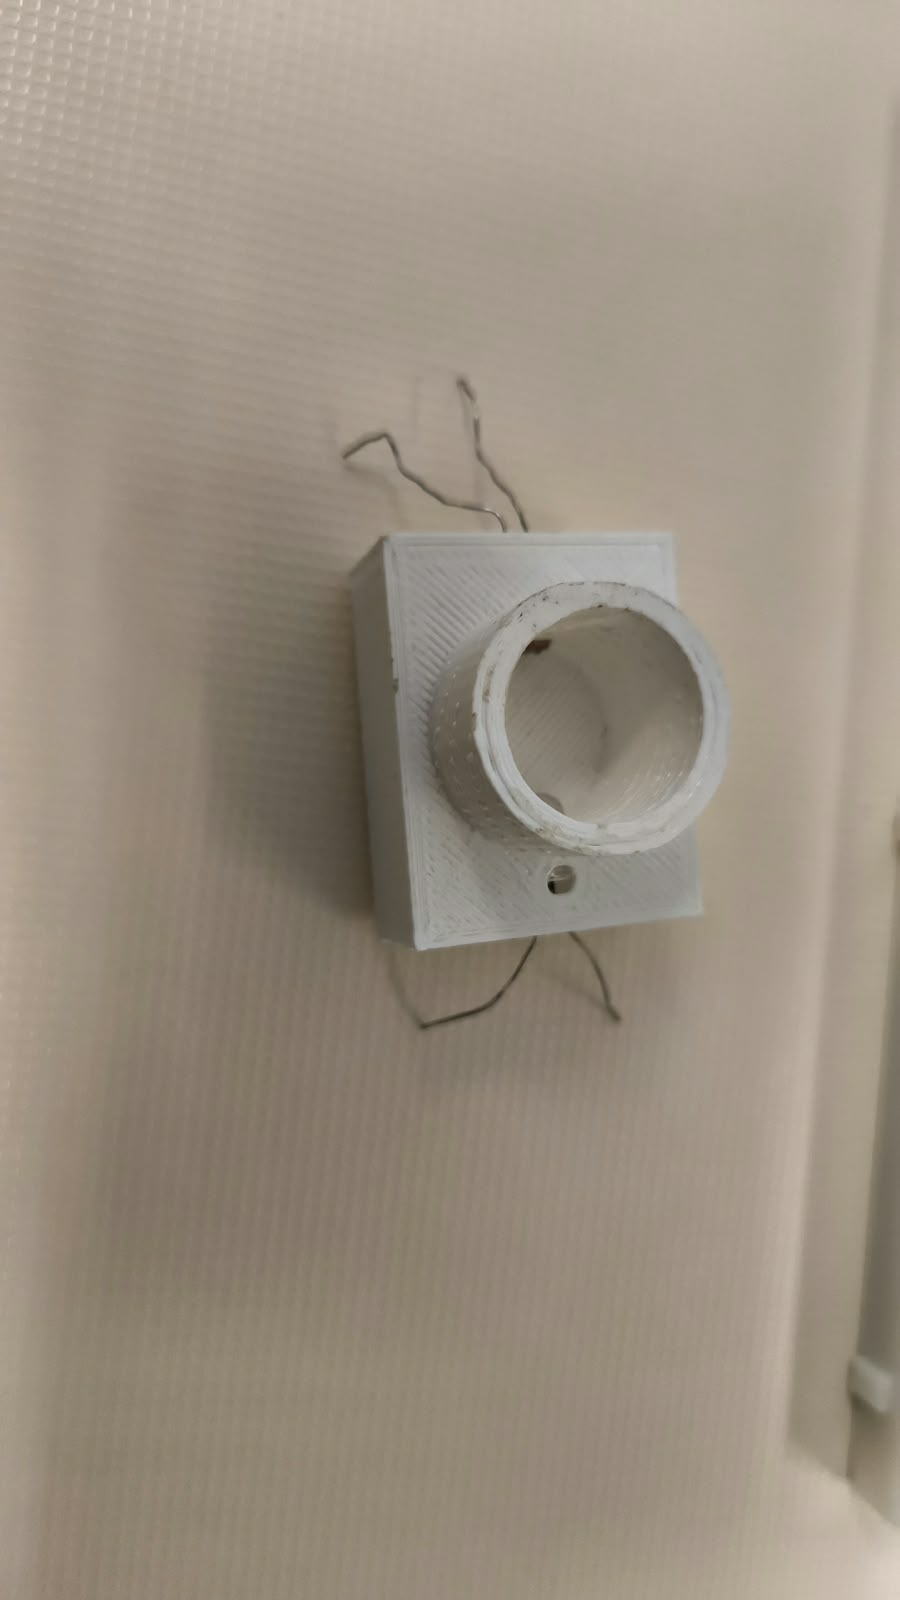
\includegraphics[width=\linewidth,trim=250 400 150 350,clip]{sensor_pulsometro.jpeg}
\end{minipage}\hfill
\begin{minipage}[c]{0.66\textwidth}
\small
Carcasa impresa en 3D con un alojamiento cilíndrico para el dedo y \textbf{cuatro hilos}
sin conectar (dos arriba y dos abajo), sin placa de acondicionamiento. Identificado en M0:
\begin{itemize}[leftmargin=1.2em,itemsep=1pt,topsep=2pt]
  \item \textbf{emisor}: LED blanco ($V_F \approx \qty{3}{V}$, fuera del rango de la prueba de
        diodo del multímetro);
  \item \textbf{detector}: LDR (fotorresistencia): resistencia simétrica, de
        \qty{250}{\kilo\ohm} a oscuras a \qty{0.3}{\kilo\ohm} con el LED y sin dedo;
        $\approx \qty{4}{\kilo\ohm}$ con el dedo.
\end{itemize}
La hipótesis inicial (LED IR + fototransistor) era incorrecta; por eso M0 se hizo antes de
montar nada.
\end{minipage}
\caption{Pulsómetro del laboratorio y sus componentes.}
\label{fig:sensor}
\end{figure}

% ======================================================================
\section{Arquitectura del sistema}

\begin{figure}[H]
\centering
\begin{tikzpicture}[node distance=0.55cm and 0.55cm, font=\small]
  \node[block] (adc) {ADC + Timer1\\\qty{500}{Hz}\\\scriptsize M3};
  \node[block, left=of adc] (det) {Detector de\\latidos, RR\\\scriptsize M5};
  \node[block, left=of det] (hrv) {BPM, HRV\\\scriptsize M6};
  \node[block, left=of hrv] (est) {Estado\\\scriptsize M7};
  \node[block, left=of est] (out) {Salidas\\serie / LCD / RGB\\\scriptsize M4, M8};
  \node[hwblock, above=1.3cm of adc] (acon) {Acondic.\\HPF + amp + LPF\\\scriptsize M2};
  \node[hwblock, left=of acon] (exc) {Excitación\\y detección\\\scriptsize M1};
  \node[hwblock, left=of exc] (sen) {Sensor\\PPG};
  \node[pcblock, below=1.1cm of out] (pc) {PC: Python\\visor + registro\\\scriptsize M4};

  \draw[arr] (sen) -- (exc);
  \draw[arr] (exc) -- node[above,lab]{$V_s$} (acon);
  \draw[arr] (acon) -- node[right,lab]{A0} (adc);
  \draw[arr] (adc) -- (det);
  \draw[arr] (det) -- (hrv);
  \draw[arr] (hrv) -- (est);
  \draw[arr] (est) -- (out);
  \draw[arr] (out) -- node[right,lab]{USB serie \qty{115200}{baud}} (pc);

  \begin{scope}[on background layer]
    \node[draw=accent, dashed, rounded corners, inner sep=6pt, fit=(adc)(det)(hrv)(est)(out),
          label={[lab]below right:Arduino Nano (ATmega328P)}] {};
  \end{scope}
\end{tikzpicture}
\caption{Diagrama de bloques. Naranja: hardware analógico; azul: firmware del
microcontrolador; verde: software en el PC.}
\label{fig:bloques}
\end{figure}

Decisiones principales:
\begin{itemize}[leftmargin=1.2em,itemsep=2pt,topsep=2pt]
  \item \textbf{Todo el procesado en el Arduino.} El PC solo visualiza y registra. Así el
        sistema funciona de forma autónoma con LCD y LED RGB (M8) y el trabajo se centra en el
        microcontrolador, que es el núcleo de la asignatura.
  \item \textbf{Muestreo por interrupción de temporizador} (Timer1), no con
        \texttt{delay()}: el periodo de muestreo fijo es imprescindible para medir intervalos
        RR con precisión de milisegundos.
  \item \textbf{Acondicionamiento analógico} con un TL082 (el único operacional disponible)
        alimentado a \qty{\pm 12}{V} desde la fuente doble del laboratorio. El plan inicial
        preveía un MCP6004 \emph{rail-to-rail} a \qty{5}{V}.
  \item \textbf{Visor en Python con PySerial + Tkinter}, las mismas herramientas que el
        material complementario de la asignatura.
\end{itemize}

% ======================================================================
\Needspace{24\baselineskip}
\section{Plan modular}

\begin{table}[H]
\centering\small
\caption{Resumen de módulos. Cada uno depende solo de los anteriores marcados.}
\label{tab:modulos}
\begin{tabularx}{\textwidth}{clXc}
\toprule
Mód. & Nombre & Entregable & Depende de \\
\midrule
M0 & Identificación del sensor   & Pinout y tipo de componentes                    & - \\
M1 & Excitación y detección      & $V_s$ con pulso visible en osciloscopio         & M0 \\
M2 & Acondicionamiento analógico & Onda de 1-3\,V p-p centrada en la mitad del ADC & M1 \\
M3 & Adquisición                 & Muestras a \qty{500}{Hz} exactos por serie      & - \\
M4 & Visor en tiempo real (PC)   & Gráfica en vivo + registro CSV                  & M3 \\
M5 & Detección de latidos y BPM  & Intervalos RR y BPM                             & M2, M3 \\
M6 & HRV                         & RMSSD, SDNN, rechazo de artefactos              & M5 \\
M7 & Indicador de estado         & Calibración + \{relajado, normal, estrés\}      & M6 \\
M8 & Salidas autónomas (opcional)& LCD 16x2 y LED RGB                              & M6 \\
M9 & Validación y medidas        & Tablas y figuras para el informe                & M5-M7 \\
\bottomrule
\end{tabularx}
\end{table}

M3 y M4 no dependen del hardware analógico: pueden desarrollarse en paralelo con M1-M2 usando
un potenciómetro o un generador de señales en A0.

% ----------------------------------------------------------------------
\subsection{M0: Identificación del sensor}

\modinfo{Determinar qué es cada uno de los cuatro hilos y qué tipo de emisor y detector
contiene el pulsómetro.}
{Tabla de pinout (hilo, color o posición, componente, terminal) y fotografía anotada.}
{Cada par de hilos identificado y comprobado en funcionamiento (LED encendido, detector
responde a la luz).}
{Tema 2 (circuitos digitales, diodos), Tema 10 (dispositivos).}

\textbf{Procedimiento} (multímetro en modo diodo y en óhmetro):
\begin{enumerate}[leftmargin=1.4em,itemsep=2pt,topsep=2pt]
  \item Medir en modo diodo todas las parejas de hilos en ambos sentidos y anotar.
  \item El par que marque una caída de tensión en un solo sentido y además se ilumine es el
        LED. La luz IR no se ve a simple vista, pero sí con la cámara frontal del móvil.
  \item Con el par restante, medir resistencia con el dedo dentro y fuera, a oscuras y con
        luz, y clasificar según la Tabla~\ref{tab:m0}.
  \item Marcar los hilos (cinta de colores) y soldarlos a una tira de pines para la
        \emph{protoboard}.
\end{enumerate}

\textbf{Resultado (17/11/2026).} El emisor se enciende pero el modo diodo marca fuera de rango:
es un LED blanco ($V_F \approx \qty{3}{V}$). El detector no tiene comportamiento de diodo y su
resistencia es simétrica y depende de la luz: es una LDR. Medidas: \qty{250}{\kilo\ohm}
tapada, \qtyrange{10}{90}{\kilo\ohm} con luz de sala, \qty{0.3}{\kilo\ohm} con el LED
encendido sin dedo y $\approx \qty{4.0}{\kilo\ohm}$ con el dedo (punto de trabajo).

\begin{table}[H]
\centering\small
\caption{Identificación de componentes con el multímetro.}
\label{tab:m0}
\begin{tabularx}{\textwidth}{lXX}
\toprule
Componente & Modo diodo & Óhmetro / luz \\
\midrule
LED infrarrojo  & $\approx$ \qtyrange{1.0}{1.4}{V} en un sentido, abierto en el otro & Brilla en la cámara del móvil \\
LED rojo        & $\approx$ \qtyrange{1.7}{2.2}{V} en un sentido; brillo visible débil & - \\
Fotodiodo (Si)  & $\approx$ \qtyrange{0.5}{0.7}{V} en un sentido & Corriente/tensión con luz \\
Fototransistor  & Abierto o muy alto en ambos sentidos & $R_{CE}$ cae mucho con luz (en un sentido) \\
LDR             & Sin comportamiento de diodo & Resistencia simétrica, de M$\Omega$ a k$\Omega$ con luz \\
\bottomrule
\end{tabularx}
\end{table}

% ----------------------------------------------------------------------
\subsection{M1: Excitación y detección}

\modinfo{Alimentar el LED con corriente controlada y polarizar el fotodetector para obtener
una tensión $V_s$ proporcional a la luz recibida.}
{Circuito de la Figura~\ref{fig:m1} montado y caracterizado.}
{$V_s$ cerca de la mitad de la alimentación con el dedo dentro y pequeña oscilación (mV) al
ritmo del pulso.}
{Tema 2 (características eléctricas), Tema 10 (dispositivos).}

\begin{figure}[H]
\centering
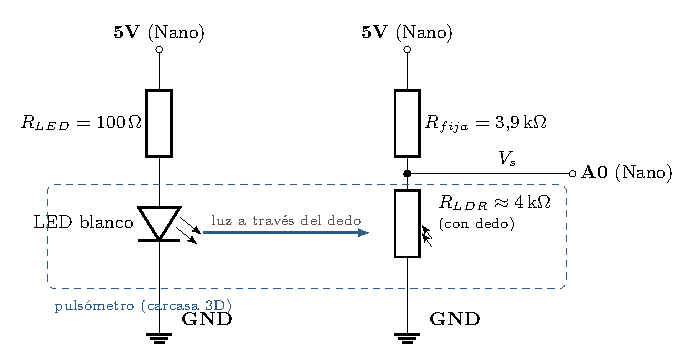
\includegraphics[width=0.62\textwidth]{paso4_divisor_ldr.pdf}
\caption{M1 construido: LED blanco con \qty{100}{\ohm} desde el \qty{5}{V} del Nano y divisor
con la LDR en la parte baja. $V_s$ sube cuando llega menos luz (más sangre).}
\label{fig:m1}
\end{figure}

\textbf{Dimensionado.}
\begin{itemize}[leftmargin=1.2em,itemsep=2pt,topsep=2pt]
  \item LED: $I = (5 - V_F)/R \approx (5 - 3{,}1)/\qty{97.1}{\ohm} \approx \qty{19.6}{mA}$,
        dentro de los \qty{20}{mA} nominales de un LED de \qty{5}{mm}. Va al \qty{5}{V} y no a
        un pin: un pin del ATmega328P no debe dar tanta corriente de forma continua.
  \item Resistencia fija del divisor: la sensibilidad
        $\partial V_s/\partial R_{LDR} = V_{CC} R/(R + R_{LDR})^2$ es máxima con
        $R = R_{LDR} \approx \qty{4}{\kilo\ohm}$. Se elige \qty{3.9}{\kilo\ohm} (E12, 99,98\,\%
        del óptimo), y además $V_s \approx V_{CC}/2$.
  \item Medido: $V_s = \qty{0.37}{V}$ sin dedo y 2,5-\qty{2.7}{V} con el dedo. Pulso de
        $\approx \qty{9}{mV}$ p-p, apenas 2 escalones del ADC (\qty{4.9}{mV}): hace falta
        amplificar unas 100 veces.
\end{itemize}

% ----------------------------------------------------------------------
\subsection{M2: Acondicionamiento analógico}

\modinfo{Quitar la componente DC de $V_s$, amplificar la AC unas 100 veces, filtrar el
ruido y llevar la señal al rango del ADC.}
{Placa de acondicionamiento (Figura~\ref{fig:amp}) con la salida conectada a A0.}
{En A0: onda de pulso limpia de 1-3\,V pico a pico, sin saturar, con ruido de \qty{50}{Hz}
inapreciable.}
{Tema 3 (convertidores A/D), Tema 10 (dispositivos).}

\textbf{Por qué este diseño.} El único operacional disponible era el TL082 (dos
amplificadores, entrada JFET). No sirve a \qty{5}{V}: su entrada en modo común empieza unos
\qty{4}{V} por encima de $V_-$ y su salida no se acerca a menos de $\approx \qty{1.5}{V}$ de
cada alimentación. Se alimenta a \qty{\pm 12}{V} con la fuente doble del laboratorio
(DF1731SB, dos canales en serie, COM unido al GND del Nano). Así todas las etapas se refieren a
\qty{0}{V} y no hace falta tensión de referencia. Como la salida podría llegar a
\qty{\pm 10}{V}, al final se desplaza la señal a la mitad de \qty{5}{V} y se protege A0.

\begin{figure}[H]
\centering
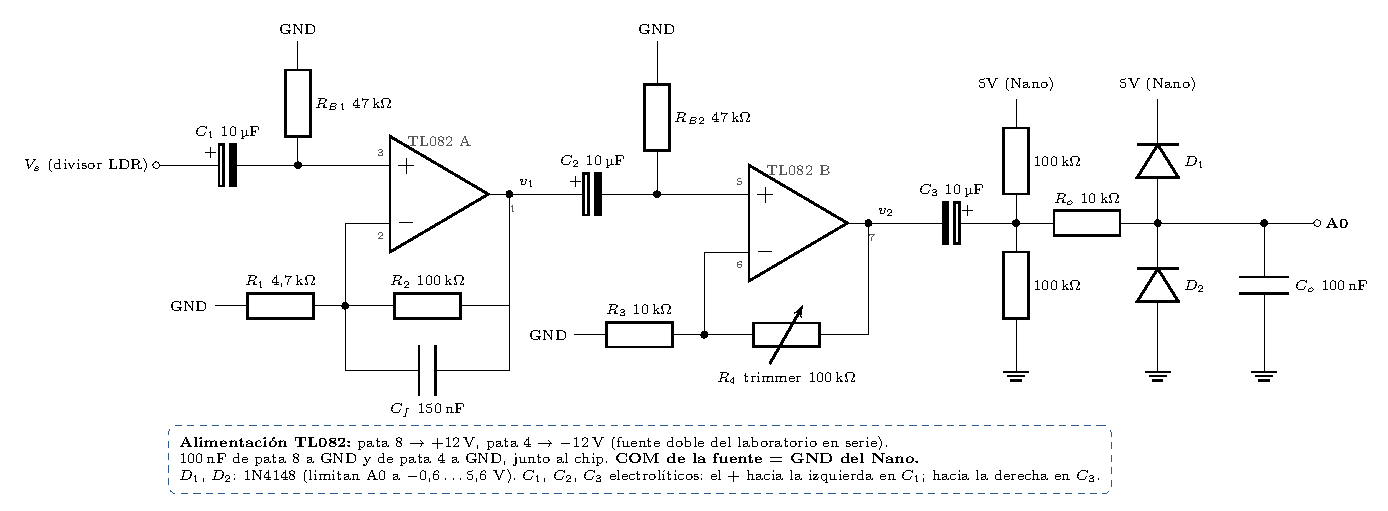
\includegraphics[width=\textwidth]{m2_tl082.pdf}
\caption{M2 construido: dos etapas no inversoras con acoplamiento en alterna (TL082 A y B) y
etapa de salida con desplazamiento a la mitad de \qty{5}{V}, diodos de protección y filtro
antialiasing.}
\label{fig:amp}
\end{figure}

\begin{table}[H]
\centering\small
\caption{Parámetros del acondicionamiento con los valores medidos de los componentes.}
\label{tab:m2}
\begin{tabular}{lll}
\toprule
Parámetro & Expresión & Valor \\
\midrule
Paso alto etapa 1 & $1/(2\pi R_{B1} C_1)$, \qty{47.3}{\kilo\ohm}, \qty{10.2}{\micro\farad} & \qty{0.33}{Hz} \\
Ganancia etapa 1 & $1 + R_2/R_1$, \qty{99.2}{\kilo\ohm}/\qty{4.6}{\kilo\ohm} & 22,6 \\
Paso bajo etapa 1 & $1/(2\pi R_2 C_f)$, $C_f = \qty{147}{\nano\farad}$ & \qty{10.9}{Hz} \\
Paso alto etapa 2 & $1/(2\pi R_{B2} C_2)$, \qty{46.2}{\kilo\ohm}, \qty{9.34}{\micro\farad} & \qty{0.37}{Hz} \\
Ganancia etapa 2 & $1 + R_4/R_3$, \qty{19.9}{\kilo\ohm}/\qty{9.79}{\kilo\ohm} & 3,03 \\
Ganancia total & $G_1 G_2$ & 68,5 \\
Paso alto de salida & $1/(2\pi (\qty{98.2}{\kilo\ohm}/2) C_3)$, $C_3 = \qty{11.25}{\micro\farad}$ & \qty{0.29}{Hz} \\
Antialiasing & $1/(2\pi R_o C_o)$, \qty{9.8}{\kilo\ohm}, \qty{100}{\nano\farad} & \qty{162}{Hz} ($< \qty{250}{Hz}$) \\
\bottomrule
\end{tabular}
\end{table}

\begin{itemize}[leftmargin=1.2em,itemsep=2pt,topsep=2pt]
  \item \textbf{Banda útil.} El pulso va de 40 a \qty{200}{BPM} (\qtyrange{0.67}{3.3}{Hz})
        con armónicos hasta unos \qty{10}{Hz}. La banda \qtyrange{0.33}{10.9}{Hz} los conserva y
        quita la DC, la deriva lenta y el ruido de red.
  \item \textbf{Por qué dos etapas.} El offset del TL082 (hasta \qty{15}{mV}) por una ganancia
        de 68 llevaría la salida a \qty{1}{V}. Con la ganancia repartida, el acoplamiento en
        alterna de la etapa 2 quita el offset amplificado de la etapa 1.
  \item \textbf{Ajuste.} $G_2$ con un potenciómetro de \qty{100}{\kilo\ohm} entre las patas 6
        y 7. Con $G_2 = 1$ el pulso medía 0,5-\qty{0.6}{V} p-p en A0; con $G_2 = 3{,}03$,
        1,5-\qty{2}{V} p-p, con margen frente a \qty{0}{V} y \qty{4.7}{V}.
  \item \textbf{Salida.} $C_3$ y el divisor de $2\times\qty{98.2}{\kilo\ohm}$ desde el
        \qty{5}{V} del Nano centran la señal en \qty{2.35}{V}: la mitad de los \qty{4.7}{V} que
        da el USB tras su diodo. El ADC usa esa misma tensión como referencia, así que queda
        en el centro de escala (ADC $\approx 512$) sea cual sea la tensión del USB. Los
        1N4148 limitan A0 a $-0{,}6\ldots\qty{5.6}{V}$ y $R_o$ limita la corriente.
  \item \textbf{Saturación al meter o sacar el dedo}: la etapa satura $\approx\qty{8}{s}$
        hasta que se cargan $C_1$-$C_3$. Es el precio de la ganancia; el firmware lo detecta
        (ADC en 0 o 1023) y reaprende.
  \item También funciona a \qty{\pm 5}{V} (las señales están cerca de \qty{0}{V}), pero se
        mantiene \qty{\pm 12}{V}, donde el fabricante garantiza las características.
\end{itemize}

% ----------------------------------------------------------------------
\subsection{M3: Adquisición por interrupción}

\modinfo{Muestrear A0 a exactamente \qty{500}{Hz} mediante interrupción del Timer1 y
almacenar las muestras en un buffer circular.}
{Sketch de prueba que envía las muestras por el puerto serie.}
{Osciloscopio en el pin de depuración D12: periodo de \qty{2.000}{ms}, la ISR dura menos de
\qty{200}{\micro s}; contador de secuencia sin saltos durante \qty{10}{min}.}
{Tema 8 (temporizadores, interrupciones, ADC), Tema 7 (memoria SRAM), Tema 9.}

\Needspace{22\baselineskip}
\textbf{Configuración del Timer1 en modo CTC:}
\[
  f_s = \frac{f_{clk}}{N\,(1 + \mathrm{OCR1A})} = \frac{\qty{16}{MHz}}{64\cdot(1 + 499)} = \qty{500}{Hz}.
\]

\begin{lstlisting}[language=C++]
void setupTimer1() {
  noInterrupts();
  TCCR1A = 0;
  TCCR1B = (1 << WGM12) | (1 << CS11) | (1 << CS10); // CTC, prescaler 64
  OCR1A  = 499;                                       // 16 MHz / 64 / 500 = 500 Hz
  TIMSK1 = (1 << OCIE1A);                              // interrupción por comparación A
  interrupts();
}

ISR(TIMER1_COMPA_vect) {
  buf[head] = analogRead(A0);          // ~110 us con el prescaler por defecto del ADC
  head = (head + 1) & (BUF_LEN - 1);   // buffer circular, BUF_LEN potencia de 2
}
\end{lstlisting}

\begin{itemize}[leftmargin=1.2em,itemsep=2pt,topsep=2pt]
  \item El procesado (detector, HRV) se hace en \texttt{loop()} leyendo del buffer; la ISR
        solo adquiere. Nunca usar \texttt{Serial} dentro de la ISR.
  \item Memoria: buffer de 256 muestras \texttt{uint16\_t} = \qty{512}{B} de los
        \qty{2}{kB} de SRAM del ATmega328P. Variables compartidas con la ISR declaradas
        \texttt{volatile} y leídas con interrupciones deshabilitadas.
  \item \textbf{Conflicto a tener en cuenta}: el Timer1 controla el PWM de D9 y D10. Por eso
        el LED RGB (M8) va en D3, D5 y D6.
  \item Ancho de banda serie: enviar todas las muestras a \qty{500}{Hz} en ASCII no cabe con
        holgura en \qty{115200}{baud}; al PC se envía una de cada cinco (\qty{100}{Hz}), más que
        suficiente para dibujar una señal de banda \qty{10}{Hz}.
  \item \textbf{Resultado}: \qty{500.39}{Hz} medidos con el reloj del PC (+0,08\,\%, tolerancia
        del oscilador del clon: \qty{0.6}{ms} de error en un RR de \qty{800}{ms}). 0 muestras
        perdidas en todas las pruebas, también con el firmware completo.
\end{itemize}

% ----------------------------------------------------------------------
\subsection{M4: Visor en tiempo real (PC)}

\modinfo{Representar la onda en tiempo real y registrar todos los datos para el análisis
posterior.}
{\texttt{pc/visor.py}: ventana Tkinter con gráfica \emph{matplotlib} embebida y fichero CSV
por sesión.}
{Ventana deslizante de \qty{5}{s} a $\ge 20$ fps sin retraso acumulado durante
\qty{10}{min}.}
{Información complementaria: Arduino + Python (PySerial), Tkinter.}

Contenido de la ventana: onda PPG con los latidos detectados marcados; BPM, RMSSD, SDNN y
estado en grande; tacograma (serie de intervalos RR, con los rechazados en rojo). Un hilo
lee el puerto serie y deposita las líneas en una cola; la interfaz se actualiza con
\texttt{after()} cada \qty{40}{ms} y redibuja solo las curvas (\emph{blitting}). Resultado:
20-\qty{25}{fps} sin retraso acumulado.

Añadido tras las pruebas en el laboratorio:
\begin{itemize}[leftmargin=1.2em,itemsep=2pt,topsep=2pt]
  \item Con el Nano graba siempre desde que se abre (CSV de señal, latidos y marcas de fase,
        estas con la barra espaciadora).
  \item \textbf{Perfiles}: al calibrar se pide un nombre y la línea base se guarda en
        \texttt{datos/perfiles.json}; al elegir un perfil se envía al Nano.
  \item \textbf{Modo producción} (\texttt{-{}-produccion}): pantalla oscura y limpia para
        demostraciones, fotos y vídeos, con el pulso, el estado, RMSSD, SDNN y la onda.
  \item Modo reproducción: reproduce una grabación como si llegara del Nano.
\end{itemize}

\textbf{Protocolo serie} (ASCII, una línea por mensaje, \qty{115200}{baud}):

\begin{table}[H]
\centering\small
\caption{Mensajes entre Arduino y PC.}
\label{tab:protocolo}
\begin{tabularx}{\textwidth}{llX}
\toprule
Sentido & Formato & Significado \\
\midrule
Ard $\to$ PC & \texttt{S,<t\_ms>,<adc>} & Muestra filtrada (\qty{100}{Hz}) \\
Ard $\to$ PC & \texttt{B,<t>,<rr>,<res>,<bpm>,<rmssd>,<sdnn>,<est>} & Latido: RR, resultado del rechazo (0 válido, 1 sin RR, 2 fuera de rango, 3 artefacto), métricas con un decimal y estado (0 sin calibrar, 1 calibrando, 2 relajado, 3 normal, 4 estrés) \\
Ard $\to$ PC & \texttt{I,<texto>} & Información: arranque, línea base, calibración, estadísticas \\
PC $\to$ Ard & \texttt{c} / \texttt{r} & Iniciar calibración / reiniciar detector y HRV \\
PC $\to$ Ard & \texttt{b<hr0}$\times$\texttt{10>,<rmssd0}$\times$\texttt{10>} & Cargar la línea base de un perfil \\
\bottomrule
\end{tabularx}
\end{table}

% ----------------------------------------------------------------------
\subsection{M5: Detección de latidos y BPM}

\modinfo{Detectar cada latido, medir el intervalo entre latidos (RR) y calcular BPM.}
{Módulo \texttt{detector} del firmware.}
{Señal sintética a 60, 72 y \qty{120}{BPM}: error $\le \qty{1}{BPM}$. Con el dedo: error
$\le \qty{2}{BPM}$ frente a una referencia; ningún latido perdido ni duplicado en
\qty{2}{min} de reposo. (El conteo manual resultó demasiado impreciso; se usó una app de
pulso del móvil.)}
{Tema 5 (máquinas de estados), Tema 4 (aritmética entera), Tema 6 (registros).}

\begin{figure}[H]
\centering
\begin{tikzpicture}[node distance=0.45cm, font=\small]
  \node[block, minimum width=1.6cm] (s1) {ADC\\\qty{500}{Hz}};
  \node[block, right=of s1, minimum width=1.6cm] (s2) {Media\\móvil 10};
  \node[block, right=of s2, minimum width=1.6cm] (s3) {Umbral\\adaptativo};
  \node[block, right=of s3, minimum width=1.6cm] (s4) {Máquina\\de estados};
  \node[block, right=of s4, minimum width=1.6cm] (s5) {Máxima\\pendiente};
  \node[block, right=of s5, minimum width=1.6cm] (s6) {RR validado\\(M6)};
  \foreach \i/\j in {s1/s2,s2/s3,s3/s4,s4/s5,s5/s6} \draw[arr] (\i) -- (\j);
\end{tikzpicture}
\caption{Cadena de procesado por muestra.}
\label{fig:cadena}
\end{figure}

\begin{enumerate}[leftmargin=1.4em,itemsep=2pt,topsep=2pt]
  \item \textbf{Media móvil de 10 muestras.} Con $f_s = \qty{500}{Hz}$ la ventana dura
        exactamente \qty{20}{ms}, un periodo de red: su respuesta en frecuencia tiene ceros en
        \qty{50}{Hz} y sus múltiplos. Elimina el ruido de red con una suma y una resta por
        muestra.
  \item \textbf{Umbral adaptativo latido a latido}: $u = v + 0{,}6\,(p - v)$, con $p$ y $v$
        medias exponenciales ($\alpha = 0{,}25$) del pico y del valle de cada latido aceptado.
        Si pasan 1,5 RR medios sin latido (la amplitud ha bajado de golpe, por ejemplo al
        cambiar la presión del dedo), $p$ decae hacia $v$ con $\tau = \qty{1}{s}$.
  \item \textbf{Máquina de estados} (Figura~\ref{fig:fsm}). Exige cruce de subida del umbral,
        amplitud mínima (\qty{22}{LSB}) y relativa (40\,\% de la media). El refractario es el
        60\,\% del RR medio, entre 250 y \qty{500}{ms}: tapa la onda dícrota, y el tope evita
        que un latido perdido lo alargue y deje el detector contando la mitad de latidos.
  \item \textbf{Instante del latido: punto de máxima pendiente de subida}, con la pendiente
        medida en \qty{20}{ms} y refinada con una parábola de puntos a \qty{\pm 20}{ms}. El
        plan proponía el pico, pero a ritmo alto la onda dícrota se junta con él, la cima se
        achata y su instante baila: en una prueba de estrés a $\approx\qty{100}{BPM}$ el RMSSD
        salía 67 ms con el pico y 37 ms con la pendiente (en reposo coinciden).
  \item \textbf{Saturación} (ADC $\le 3$ o $\ge 1020$, dedo entrando o saliendo) y
        \qty{3}{s} sin latido: vuelve a APRENDIZAJE (\qty{2}{s} para estimar pico y valle).
\end{enumerate}

\begin{figure}[H]
\centering
\begin{tikzpicture}[shorten >=1pt, node distance=3.6cm, on grid, auto, font=\small,
                    every state/.style={draw=navy, fill=softblue, thick, minimum size=1.75cm, align=center, font=\scriptsize}]
  \node[state, initial, initial text={}] (A) {APRENDI-\\ZAJE};
  \node[state, right=of A] (E) {ESPERA};
  \node[state, right=of E] (S) {SUBIDA};
  \node[state, right=of S] (R) {REFRAC-\\TARIO};
  \path[arr]
    (A) edge node[above, font=\scriptsize]{\qty{2}{s}} (E)
    (E) edge node[above, align=center, font=\scriptsize]{cruce de\\subida de $u$} (S)
    (S) edge node[above, align=center, font=\scriptsize]{$y < u$, latido\\válido: RR} (R)
    (S) edge[bend left=40] node[below, font=\scriptsize]{pico no válido} (E)
    (R) edge[bend left=45] node[below, align=center, font=\scriptsize]{$t - t_{pico} > $ refractario} (E)
    (E) edge[bend right=45] node[above, align=center, font=\scriptsize]{saturación o\\\qty{3}{s} sin latido} (A);
\end{tikzpicture}
\caption{Máquina de estados del detector. El refractario mínimo limita la frecuencia máxima
a \qty{240}{BPM}.}
\label{fig:fsm}
\end{figure}

\textbf{BPM} $= 60000/\overline{RR}$, con la media de los últimos 8 RR \emph{válidos} (lo
calcula M6).

% ----------------------------------------------------------------------
\subsection{M6: Variabilidad de la frecuencia cardiaca (HRV)}

\modinfo{Calcular los índices temporales de HRV a partir de los intervalos RR válidos.}
{Módulo \texttt{hrv} del firmware (ventana de 30 latidos) y \texttt{pc/analisis.py} (registro
completo de \qty{5}{min}).}
{Señal sintética con RR alternando 800 y \qty{900}{ms}: RMSSD $= \qty{100 \pm 2}{ms}$ y SDNN
$= \qty{50.9 \pm 2}{ms}$ (ventana de 30 latidos).}
{Tema 4 (aritmética), Tema 7 (buffers en memoria).}

Para una serie de $N$ intervalos $RR_i$:
\[
  \mathrm{SDNN} = \sqrt{\frac{1}{N-1}\sum_{i=1}^{N}\left(RR_i - \overline{RR}\right)^2},
  \qquad
  \mathrm{RMSSD} = \sqrt{\frac{1}{N-1}\sum_{i=1}^{N-1}\left(RR_{i+1} - RR_i\right)^2}.
\]
SDNN mide la variabilidad global; RMSSD, la variabilidad latido a latido, ligada a la
actividad parasimpática (vagal): disminuye con el estrés y aumenta con la relajación.

\begin{itemize}[leftmargin=1.2em,itemsep=2pt,topsep=2pt]
  \item \textbf{Rechazo de artefactos}: se descarta un RR fuera de \qtyrange{300}{2000}{ms} o
        que difiera más de un \textbf{30\,\%} del último válido. Con un solo RR erróneo, RMSSD se
        dispara, así que este filtro es esencial. El plan inicial decía 20\,\%, pero la
        arritmia respiratoria real cambia el RR hasta un 25,5\,\% de un latido al siguiente:
        con 20\,\% se rechazaban 17 RR buenos de 64. Sin referencia (al arrancar), el primer RR
        solo se acepta si coincide con el siguiente; con 5 rechazos seguidos se reinicia.
        Solo se usan diferencias entre RR contiguos para el RMSSD.
  \item \textbf{Ventanas.} En el Arduino, ventana deslizante de 30 RR (unos \qty{30}{s}),
        suficiente para RMSSD según la literatura de registros ultracortos. En el PC, el
        estándar de registro corto de \qty{5}{min} para los valores del informe, más el
        diagrama de Poincaré ($RR_{i+1}$ frente a $RR_i$, con $SD1 \approx \mathrm{RMSSD}/\sqrt{2}$).
  \item \textbf{Aritmética}: RR en \texttt{uint16\_t} (ms) y varianza exacta en
        \texttt{uint32\_t},
        \[ s^2 = \frac{N\sum RR^2 - \left(\sum RR\right)^2}{N(N-1)}, \]
        sin desbordamiento: con $N \le 30$ y $RR \le \qty{2000}{ms}$,
        $N\sum RR^2 \le 3{,}6\cdot 10^9 < 2^{32}$. Una sola raíz en coma flotante por latido.
  \item \textbf{Limitación a discutir}: con PPG se mide la variabilidad del \emph{pulso}
        (PRV), no la del ECG. En reposo coinciden bien, pero con movimiento o estrés la PRV
        se desvía.
\end{itemize}

% ----------------------------------------------------------------------
\subsection{M7: Indicador de estado}

\modinfo{Clasificar el estado en \{relajado, normal, estrés\} comparando con una línea base
personal.}
{Módulo \texttt{estado} con calibración por pulsador (D2) o por comando \texttt{c}.}
{Protocolo de pruebas de M9: la tendencia del indicador coincide con la esperada.}
{Tema 5 (máquinas de estados).}

La HRV varía mucho entre personas, por lo que no se usan umbrales absolutos. Se calibra una
línea base con \qty{2}{min} en reposo sentado y al menos 60 RR ($HR_0$ medio y
$\mathrm{RMSSD}_0$ con todas las diferencias contiguas del periodo) y se clasifica por
comparación. La línea base se guarda en la EEPROM: abrir el puerto serie reinicia el Nano, y
sin ella habría que recalibrar cada vez.

\begin{table}[H]
\centering\small
\caption{Reglas de clasificación. La de estrés se cambió tras las pruebas reales.}
\label{tab:estado}
\begin{tabularx}{\textwidth}{lX}
\toprule
Estado & Condición \\
\midrule
Relajado & $\mathrm{RMSSD} \ge 1{,}15\,\mathrm{RMSSD}_0$ y $HR \le HR_0 + 5$ \\
Estrés (v1.0) & ($\mathrm{RMSSD} \le 0{,}70\,\mathrm{RMSSD}_0$ y $HR \ge HR_0 + 10$) o $\mathrm{RMSSD} \le 0{,}5\,\mathrm{RMSSD}_0$ \\
\textbf{Estrés (v2.0)} & ($HR \ge HR_0 + 10$ y $\mathrm{RMSSD} \le 1{,}15\,\mathrm{RMSSD}_0$) o $HR \ge HR_0 + 15$ o $\mathrm{RMSSD} \le 0{,}5\,\mathrm{RMSSD}_0$ \\
Normal   & en otro caso \\
\bottomrule
\end{tabularx}
\end{table}

\textbf{Por qué se cambió.} En las pruebas con cálculo mental el pulso subió 12-\qty{18}{BPM}
pero el RMSSD se quedó en 25-\qty{32}{ms} con $\mathrm{RMSSD}_0 = \qty{25}{ms}$: la regla
inicial nunca marcaba estrés. Con la nueva, una prueba rápida de prensión (apretar fuerte con
la otra mano \qty{1}{min}) da estrés a los \qty{10}{s} y la respiración lenta da relajado.

\textbf{Histéresis}: el estado mostrado solo cambia si el nuevo se mantiene durante 10
latidos consecutivos, para evitar parpadeos. Es un indicador orientativo, no una medida
clínica; así debe presentarse en el informe.

% ----------------------------------------------------------------------
\subsection{M8: Salidas autónomas (opcional)}

\modinfo{Que el sistema funcione sin PC.}
{LCD 16x2 con BPM, RMSSD y estado; LED RGB con el color del estado; LED D13 parpadeando
con cada latido.}
{Lectura coherente con el visor del PC, refresco de \qty{1}{Hz}.}
{Tema 10 (LCD, librería \texttt{LiquidCrystal}).}

\begin{center}\small
\texttt{BPM: 72\ \ \ \ RELAX}\\
\texttt{RMSSD:45 SDNN:52}
\end{center}

Colores del LED RGB: verde (relajado), azul (normal), rojo (estrés), blanco parpadeando
(calibrando). Resistencias de \qty{220}{\ohm} por canal.

% ----------------------------------------------------------------------
\subsection{M9: Banco de pruebas, validación y medidas}

\modinfo{Validar cada módulo con señales conocidas y obtener las medidas del informe.}
{Tablas de error, capturas y CSV de las sesiones del protocolo.}
{Criterios de la Tabla~\ref{tab:alcance}.}
{Práctica 2 (Arduino), propuesta \emph{Generación de una señal mediante PWM (pulso cardiaco)}.}

\textbf{Señales de prueba con RR conocidos.} En lugar del generador con un segundo Arduino
previsto, los módulos de cálculo (detector, HRV, estado) son C++ sin dependencias de Arduino y
se compilan también en el PC (\texttt{pc/test\_detector.cpp}). Se prueban con:
\begin{enumerate}[leftmargin=1.4em,itemsep=2pt,topsep=2pt]
  \item \textbf{Señales sintéticas} (\texttt{pc/sintetica.py}) a \qty{500}{Hz} con onda
        sistólica, onda dícrota, ruido de red y cuantización, y RR conocidos: 60, 72 y
        \qty{120}{BPM}, arritmia sinusoidal, RR alternando 800 y \qty{900}{ms}, latidos
        perdidos y un protocolo completo de reposo, estrés y relajación de \qty{7}{min}.
  \item \textbf{Grabaciones reales} hechas con el visor, que se reprocesan con el mismo código
        del Nano: cada cambio del firmware se comprueba con todas ellas en segundos.
\end{enumerate}

\textbf{Protocolo de medidas con el dedo} (sentado, mano y antebrazo apoyados):
\begin{enumerate}[leftmargin=1.4em,itemsep=2pt,topsep=2pt]
  \item Reposo y comparación del BPM con una referencia (app de pulso del móvil o
        pulsioxímetro).
  \item Calibración de \qty{2}{min} en reposo.
  \item Protocolo rápido con marcas de fase: \qty{1}{min} de reposo, \qty{1}{min} de prensión
        isométrica con la mano libre (estrés) y \qty{1}{min} de respiración lenta, 5\,s
        inspirando y 5\,s espirando (relajación). Más rápido y repetible que las fases de
        \qty{5}{min} previstas; el cálculo mental mueve poco el pulso y hablar altera la HRV.
  \item Registro de \qty{5}{min} en reposo para los valores de HRV del informe.
\end{enumerate}

% ======================================================================
\section{Conexionado del Arduino Nano}

\begin{table}[H]
\centering\small
\caption{Asignación de pines.}
\label{tab:pines}
\begin{tabularx}{\textwidth}{llXc}
\toprule
Pin & Dirección & Función & Módulo \\
\midrule
A0      & Entrada analógica & Señal PPG acondicionada & M2, M3 \\
5V      & Alimentación & LED del sensor (vía \qty{100}{\ohm}), divisor de la LDR y divisor de salida de M2 & M1, M2 \\
D2      & Entrada (\texttt{INPUT\_PULLUP}) & Pulsador de calibración (a GND, antirrebote de \qty{50}{ms} por software) & M7 \\
D3, D5, D6 & Salida PWM (Timer2, Timer0) & LED RGB: rojo, verde, azul & M8 \\
D8, D9, D10, D11, A1, A2 & Salida digital & LCD 16x2 en modo 4 bits: RS, E, DB4-DB7 & M8 \\
D12     & Salida & Depuración: se conmuta en la ISR para medir temporización & M3 \\
D13     & Salida & LED integrado, parpadea con cada latido & M5 \\
D0, D1  & - & Reservados para el puerto serie USB & M4 \\
GND     & Masa & Común con el COM de la fuente de \qty{\pm 12}{V} del TL082 & todos \\
\bottomrule
\end{tabularx}
\end{table}

Si el LCD disponible lleva adaptador I2C (PCF8574), se conecta a A4 (SDA) y A5 (SCL) y quedan
libres D8-D11, A1 y A2. D9 y D10 se usan solo como salidas digitales, lo que es compatible con
el Timer1 ocupado por el muestreo.

% ======================================================================
\Needspace{30\baselineskip}
\section{Lista de componentes}

\begin{table}[H]
\centering\small
\caption{Componentes necesarios.}
\label{tab:bom}
\begin{tabularx}{\textwidth}{lXcc}
\toprule
Componente & Valor / modelo (medido) & Cant. & Módulo \\
\midrule
Microcontrolador & Arduino Nano clónico (ATmega328P, bootloader antiguo) + cable USB & 1 & todos \\
Sensor & Pulsómetro del laboratorio: LED blanco + LDR & 1 & M0 \\
Amplificador operacional & TL082CP (doble, entrada JFET) & 1 & M2 \\
Fuente & Fuente doble del laboratorio DF1731SB, \qty{\pm 12}{V} (\qty{11.80}{V} / \qty{-11.75}{V}) & 1 & M2 \\
Resistencias & \qty{100}{\ohm} (LED; \qty{97.1}{\ohm}) & 1 & M1 \\
 & \qty{3.9}{\kilo\ohm} (divisor de la LDR; \qty{3.86}{\kilo\ohm}) & 1 & M1 \\
 & \qty{47}{\kilo\ohm} ($R_{B1}$, $R_{B2}$; 47,3 y \qty{46.2}{\kilo\ohm}) & 2 & M2 \\
 & \qty{4.7}{\kilo\ohm} ($R_1$; \qty{4.6}{\kilo\ohm}) & 1 & M2 \\
 & \qty{100}{\kilo\ohm} ($R_2$ y divisor de salida; 99,2, 98,2 y \qty{98.2}{\kilo\ohm}) & 3 & M2 \\
 & \qty{10}{\kilo\ohm} ($R_3$, $R_o$; 9,79 y \qty{9.8}{\kilo\ohm}) & 2 & M2 \\
 & \qty{220}{\ohm} (LED RGB) & 3 & M8 \\
Potenciómetros & \qty{100}{\kilo\ohm} ($R_4$, ajustado a \qty{19.9}{\kilo\ohm}) & 1 & M2 \\
 & \qty{10}{\kilo\ohm} (contraste LCD) & 1 & M8 \\
Condensadores & \qty{10}{\micro\farad} electrolíticos ($C_1$, $C_2$, $C_3$; 10,2, 9,34 y \qty{11.25}{\micro\farad}) & 3 & M2 \\
 & \qty{150}{\nano\farad} ($C_f$; \qty{147}{\nano\farad}) & 1 & M2 \\
 & \qty{100}{\nano\farad} ($C_o$ y desacoplo de las patas 4 y 8) & 3 & M2 \\
Diodos & 1N4148 (protección de A0) & 2 & M2 \\
Pulsador & Normalmente abierto & 1 & M7 \\
LED RGB & Cátodo común, \qty{5}{mm} & 1 & M8 \\
Display & LCD 16x2 HD44780 (paralelo o con I2C) & 1 & M8 \\
Montaje & Protoboard, cables, tira de pines, cinta para marcar hilos & - & todos \\
Instrumentos & Multímetro, fuente doble & - & M0-M9 \\
\bottomrule
\end{tabularx}
\end{table}

% ======================================================================
\Needspace{34\baselineskip}
\section{Estructura del software}

\begin{lstlisting}[language={}]
trabajo_final/
  plan/                 este documento
  firmware/
    pulso/              sketch final
      pulso.ino         setup() y loop(): orquesta los módulos, protocolo serie, EEPROM
      adquisicion.h/.cpp   Timer1, ISR, buffer circular          (M3)
      detector.h/.cpp      filtro, umbral, máquina de estados    (M5)
      hrv.h/.cpp           rechazo de RR, BPM, RMSSD, SDNN       (M6)
      estado.h/.cpp        calibración y clasificación           (M7)
    pruebas/m3_timer/   sketch de prueba de la adquisición
  pc/
    visor.py            interfaz en tiempo real, modos test y producción  (M4)
    analisis.py         HRV de una sesión, tacograma, Poincaré            (M9)
    sintetica.py        señales sintéticas con RR conocidos               (M9)
    test_detector.cpp   banco de pruebas: el firmware compilado en el PC  (M9)
    monitor_m3.py       monitor de la prueba de M3
    requirements.txt    pyserial, matplotlib, numpy
  datos/                CSV de cada sesión de medida y perfiles.json
  informe/              notas por módulo, figuras e informe
  referencias/          fotos del sensor
\end{lstlisting}

Los módulos \texttt{detector}, \texttt{hrv} y \texttt{estado} no usan nada de Arduino: el
mismo código se compila en el Nano y en el PC. Así cada cambio se prueba en segundos con las
señales sintéticas y con todas las grabaciones reales antes de cargarlo.

% ======================================================================
\Needspace{40\baselineskip}
\section{Calendario}

La fecha de entrega aún no está publicada en Moodle. El calendario supone una presentación a
mediados de diciembre (las clases terminan el 11/12) y se ajustará cuando se publique.
\textbf{Avance real}: M0-M7 y M9 quedaron hechos entre el 16 y el 23/11, por delante del
calendario; queda M8 (opcional), el informe y la presentación.

\begin{figure}[H]
\centering
\begin{ganttchart}[
    time slot format=isodate,
    x unit=0.355cm, y unit chart=0.52cm,
    hgrid, vgrid={*6{draw=none},*1{dotted}},
    title height=1,
    title label font=\scriptsize,
    bar label font=\scriptsize,
    milestone label font=\scriptsize\bfseries,
    bar/.append style={fill=softblue, draw=navy},
    bar height=0.55,
    milestone/.append style={fill=accent, draw=navy},
    group/.append style={fill=navy},
  ]{2026-11-16}{2026-12-20}
  \gantttitle{Noviembre}{15} \gantttitle{Diciembre}{20} \\
  \gantttitlelist{16,...,30}{1} \gantttitlelist{1,...,20}{1} \\
  \ganttbar{M0-M1 Sensor}{2026-11-17}{2026-11-20} \\
  \ganttbar{M2 Acondicionamiento}{2026-11-19}{2026-11-26} \\
  \ganttbar{M3 Adquisición}{2026-11-21}{2026-11-26} \\
  \ganttbar{M4 Visor PC}{2026-11-23}{2026-11-29} \\
  \ganttmilestone{Onda en el PC}{2026-11-29} \\
  \ganttbar{M5 Latidos y BPM}{2026-11-27}{2026-12-03} \\
  \ganttbar{M6 HRV}{2026-12-01}{2026-12-05} \\
  \ganttmilestone{BPM + HRV}{2026-12-05} \\
  \ganttbar{M7 Estado}{2026-12-04}{2026-12-09} \\
  \ganttbar{M8 LCD y RGB}{2026-12-07}{2026-12-10} \\
  \ganttbar{M9 Validación}{2026-12-03}{2026-12-12} \\
  \ganttbar{Informe}{2026-12-07}{2026-12-16} \\
  \ganttbar{Presentación (Canva)}{2026-12-12}{2026-12-18}
\end{ganttchart}
\caption{Planificación tentativa. Las sesiones de laboratorio del 18 y 19/11 se aprovechan
para M0-M1 con multímetro y osciloscopio.}
\label{fig:gantt}
\end{figure}

% ======================================================================
\section{Riesgos y contingencias}
\label{sec:riesgos}

\begin{table}[H]
\centering\small
\caption{Riesgos identificados y respuesta prevista.}
\label{tab:riesgos}
\begin{tabularx}{\textwidth}{>{\raggedright\arraybackslash}p{4.2cm}X}
\toprule
Riesgo & Respuesta \\
\midrule
El detector es un \textbf{fotodiodo} & Amplificador de transimpedancia con el cuarto
operacional ($U_{1D}$): $R_f = \qty{1}{\mega\ohm}$ en paralelo con \qty{10}{\nano\farad},
ánodo a $V_{ref}$; sustituye al seguidor de emisor de M1. \\
El detector es una \textbf{LDR} \emph{(ocurrió)} & Divisor con resistencia fija igual a la de la LDR con el dedo
dentro. Es lenta (decenas de ms) pero suficiente para el pulso. \\
La señal satura & Bajar $G_1$ ($R_1 = \qty{10}{\kilo\ohm}$) y $G_2$; bajar la corriente del LED. \\
La señal es muy débil & Más corriente de LED ($R_{LED} = \qty{150}{\ohm}$, $\approx \qty{25}{mA}$ desde \qty{5}{V} directo, no desde un pin); dedo caliente y bien apoyado; más ganancia. \\
Ruido de \qty{50}{Hz} & Media móvil de 20 ms, cables cortos, carcasa cerrada a la luz ambiente. \\
Artefactos de movimiento & Mano y antebrazo apoyados; rechazo de RR (criterio del 30\,\%). \\
Solo hay LM324 o LM358 & Su salida no llega a \qty{5}{V} (máx. $\approx \qty{3.5}{V}$): limitar la amplitud a \qty{\pm 0.8}{V} alrededor de \qty{2.5}{V}. \\
Solo hay \textbf{TL082} \emph{(ocurrió)} & Alimentarlo a \qty{\pm 12}{V} con la fuente del laboratorio, etapas referidas a GND y desplazamiento final al rango del ADC con protección por diodos. \\
Etapa en lazo abierto \emph{(ocurrió)} & Faltaba $R_4$: la salida saturaba y oscilaba. Medir resistencias siempre con la fuente apagada. \\
Cambios bruscos de amplitud \emph{(ocurrió)} & Umbral con decaimiento y refractario con tope. \\
El indicador de estrés no responde \emph{(ocurrió)} & Regla basada en el pulso, probada con prensión isométrica. \\
Falta de tiempo & Las prioridades de la Tabla~\ref{tab:alcance} permiten cortar por M7/M8 con un sistema completo de BPM + HRV. \\
\bottomrule
\end{tabularx}
\end{table}

% ======================================================================
\section{Notas para el informe y la presentación}

\textbf{Qué guardar en cada módulo} (en \texttt{datos/} e \texttt{informe/figuras/}):
\begin{itemize}[leftmargin=1.2em,itemsep=2pt,topsep=2pt]
  \item M0-M1: foto del sensor con hilos marcados, tabla de pinout, $V_s$ en el osciloscopio.
  \item M2: capturas en $V_s$, $v_1$ y A0 (efecto de cada etapa); valores finales de los
        trimmers; esquema definitivo.
  \item M3: captura del pin de depuración (periodo y duración de la ISR).
  \item M4: captura de pantalla del visor en funcionamiento.
  \item M5-M6: tabla de validación con señales sintéticas (esperado frente a medido) y
        comparación con conteo manual.
  \item M7-M9: CSV de cada fase del protocolo; tacogramas, diagramas de Poincaré y tabla de
        BPM, RMSSD y SDNN por fase.
  \item Foto del montaje completo y vídeo corto funcionando (para la presentación).
\end{itemize}

\textbf{Guion de la presentación en Canva} (unas 10 diapositivas):
\begin{enumerate}[leftmargin=1.4em,itemsep=1pt,topsep=2pt]
  \item Título y objetivo.
  \item Qué es la PPG y qué miden BPM y HRV.
  \item Diagrama de bloques (Figura~\ref{fig:bloques}).
  \item Sensor y acondicionamiento: esquema y señal antes y después.
  \item Adquisición: Timer1 e interrupciones.
  \item Detector de latidos: máquina de estados.
  \item HRV e indicador de estado.
  \item Validación con señales sintéticas.
  \item Resultados del protocolo (reposo, respiración lenta, estrés, ejercicio).
  \item Demostración en directo o vídeo; conclusiones y mejoras.
\end{enumerate}

% ======================================================================
\section{Referencias}

\begin{enumerate}[leftmargin=1.6em,itemsep=2pt,topsep=2pt,label={[\arabic*]}]
  \item Task Force of the European Society of Cardiology and the North American Society of
        Pacing and Electrophysiology. \emph{Heart rate variability: standards of measurement,
        physiological interpretation and clinical use}. Circulation 93(5), 1043-1065, 1996.
  \item J. Allen. \emph{Photoplethysmography and its application in clinical physiological
        measurement}. Physiological Measurement 28(3), R1-R39, 2007.
  \item F. Shaffer, J. P. Ginsberg. \emph{An overview of heart rate variability metrics and
        norms}. Frontiers in Public Health 5:258, 2017.
  \item M. L. Munoz et al. \emph{Validity of (ultra-)short recordings for heart rate
        variability measurements}. PLoS ONE 10(9): e0138921, 2015.
  \item A. Schäfer, J. Vagedes. \emph{How accurate is pulse rate variability as an estimate of
        heart rate variability?} International Journal of Cardiology 166(1), 15-29, 2013.
  \item Microchip. \emph{ATmega328P datasheet} (temporizadores, ADC, interrupciones).
  \item Texas Instruments. \emph{TL08xx JFET-input operational amplifiers datasheet}.
  \item Material de la asignatura: Temas 8, 9 y 10; \emph{Arduino Python} y
        \emph{Tkinter Python} (Información complementaria).
\end{enumerate}

\end{document}
